\section{Merging Heuristics}
\indent Unfortunately, although the label-swapping algorithm yields perfectly satisfying graphs, it often doesn't sufficiently disguise a given graph.  In this section, we present a heuristic, called \emph{adjacency group merges} (or simply \emph{merges}) that further randomizes a given graph, but is not guaranteed to maintain the same k-neighborhood.

\begin{definition}
\noindent A \emph{merging} of a graph's adjacency groups combines similar adjacency groups into larger groups containing the union of their nodes based on their \emph{difference}. The difference between adjacency groups $A$ and $B$ is the size of the symmetric difference of $N_k(v)$ and $N_k(u)$, for $v \in A$ and $u \in B$. 
\end{definition}

\subsection{Non-Deterministic Merging}

%\indent This process takes in two values \emph{maximum difference} and %\emph{}

\begin{figure}[htb]
  \label{merge_k_2}
  \centering
  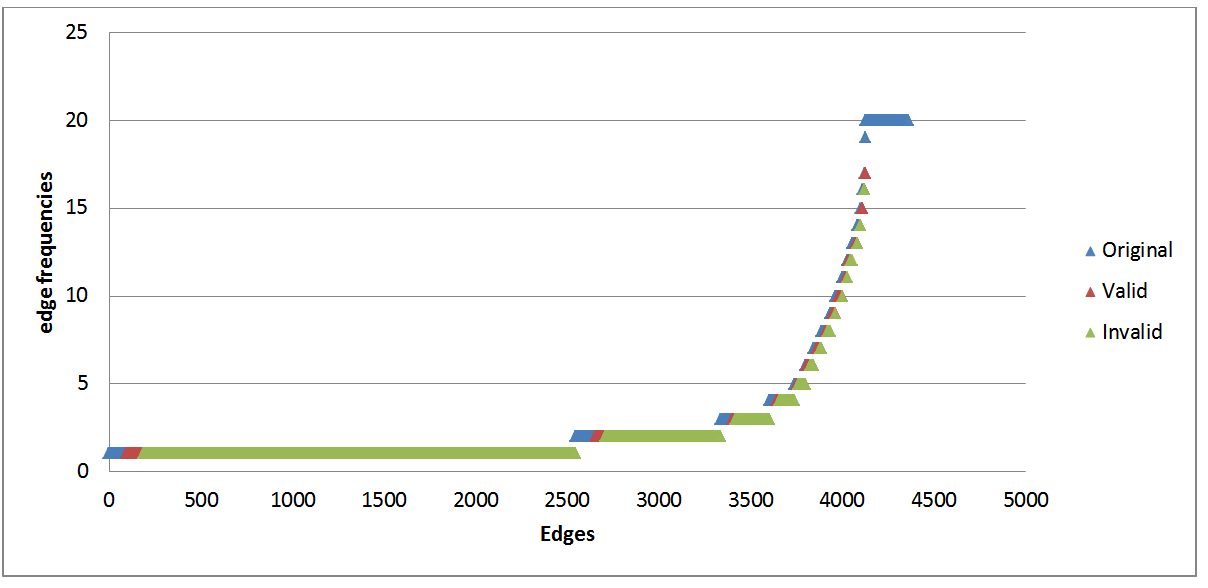
\includegraphics[scale=0.4]{mu=0_1-k=2-non-det-merge-5.png}
  \caption{The results of the non-deterministics merging where mu=0.1 and k=2}
  \label{fig:merge_k_2}
\end{figure}

\begin{figure}[htb]
  \label{merge_k_5}
  \centering
  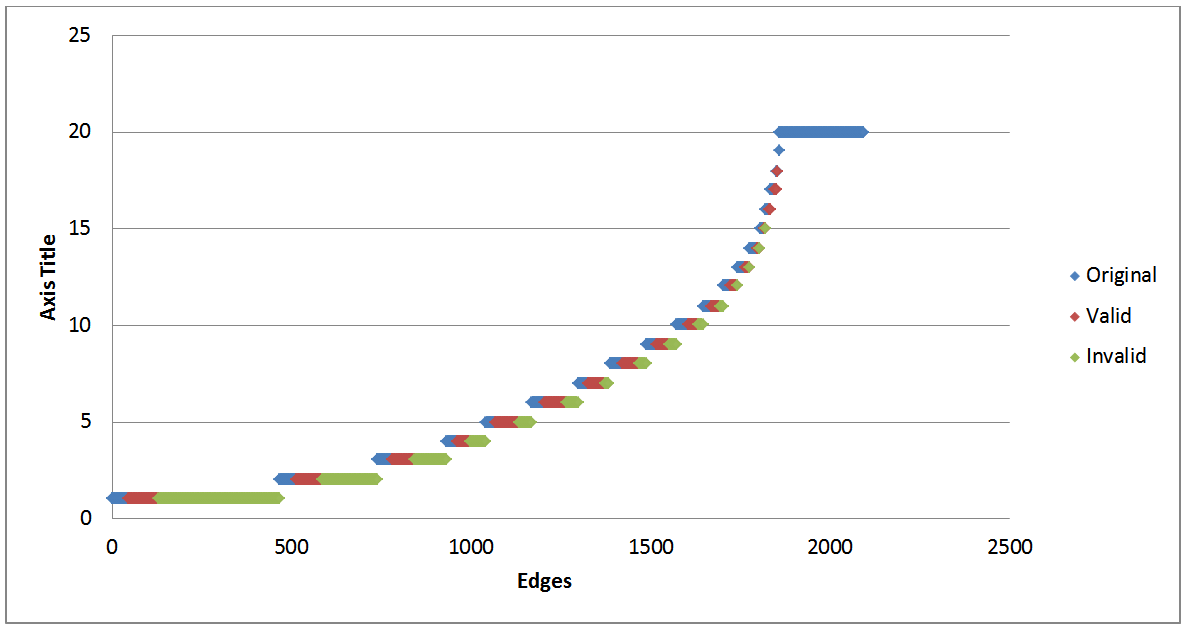
\includegraphics[scale=0.4]{mu=0_1-k=5-non-det-merge-5.png}
  \caption{The results of the non-deterministics merging where mu=0.1 and k=5}
  \label{fig:merge_k_5}
\end{figure}

\begin{definition}
An \emph{adjacency group merging} maps every pair of nodes to  the differencence value between their adjacency groups and merges adjacency groups of the first n that have not been involved in a previous merge.
\end{definition}

\begin{figure}[htb]
	\begin{algorithmic}
		\renewcommand{\algorithmicrequire}{\textbf{Input:}}
		\renewcommand{\algorithmicensure}{\textbf{Output:}}
		\Require {graph $G=(V,E)$, k-neighborhoods $K= \{k_{1}, k_{2}, ...\}$, adjecency groups $A=\{a_{1}, a_{2}, ...\}$, limit L}
		\Ensure {adjecency groups $A'$}
		\ForAll {$v \in V$}
			\ForAll {$w \in W$ where $v \neq w$}
				\State {find $Diff(A(v),A(w))$}
			\EndFor
		\EndFor
		\ForAll {$(v,w,d) \in V \times V \times {\mathbb Z}$ sorted by $d = Diff(A(v),A(w))$ where $v \neq w$}
			\State {$n = 0$}
		\EndFor
		\If {$not_merged(A(v))$ and $not_merged(A(w))$}
			\State {$merge(A(v),A(w))$}
			\State {$mark_as_merged(A(v))$}
			\State {$mark_as_merged(A(w))$}
			\State {$n++$}
			\If {$n == L$}
				\State {break}
			\EndIf
		\EndIf
	\end{algorithmic}
	\caption{Pseudocode for the Merging Heuristic Algorithm.}
	\label{fig:merging}
\end{figure}
